\subsection{Aufstellen von Funktionsgleichungen}
Viele Sachverhalte lassen sich durch Funktionen beschreiben: Die Form einer Achterbahn, die Bewegung eines Roboters, die Flugbahn eines Golfballes, die Geschwindigkeit einer Autokolonne u.v.m. Manchmal lassen sich diese aus zugrundeliegenden Gesetzmässigkeiten herleiten. In anderen Fällen kennt man aufgrund einer Messreihe oder aus logischen Überlegungen einige Funktionswerte oder spezielle Punkte und sucht nach einer Funktion, welche die gesetzten Bedingungen erfüllt. Wir gehen in diesem Kapitel also gewissermassen den umgekehrten Weg im Vergleich zum Kapitel davor. Vorgegebene Informationen über Eigenschaften eines Funktionsgraphen geben uns Hinweise über die Gleichung der Funktion und deren Ableitung. Daraus rekonstruieren wir die Funktionsgleichung.

\begin{bsp}
	{Funktionsgleichung bestimmen}{}
	Der Graph einer Polynomfunktion 3. Grades hat im Punkt $P=(2|1)$ ein lokales Minimum und in $Q=(1|3)$ einen Wendepunkt. Wie lautet die Funktionsgleichung?

	\begin{center}
		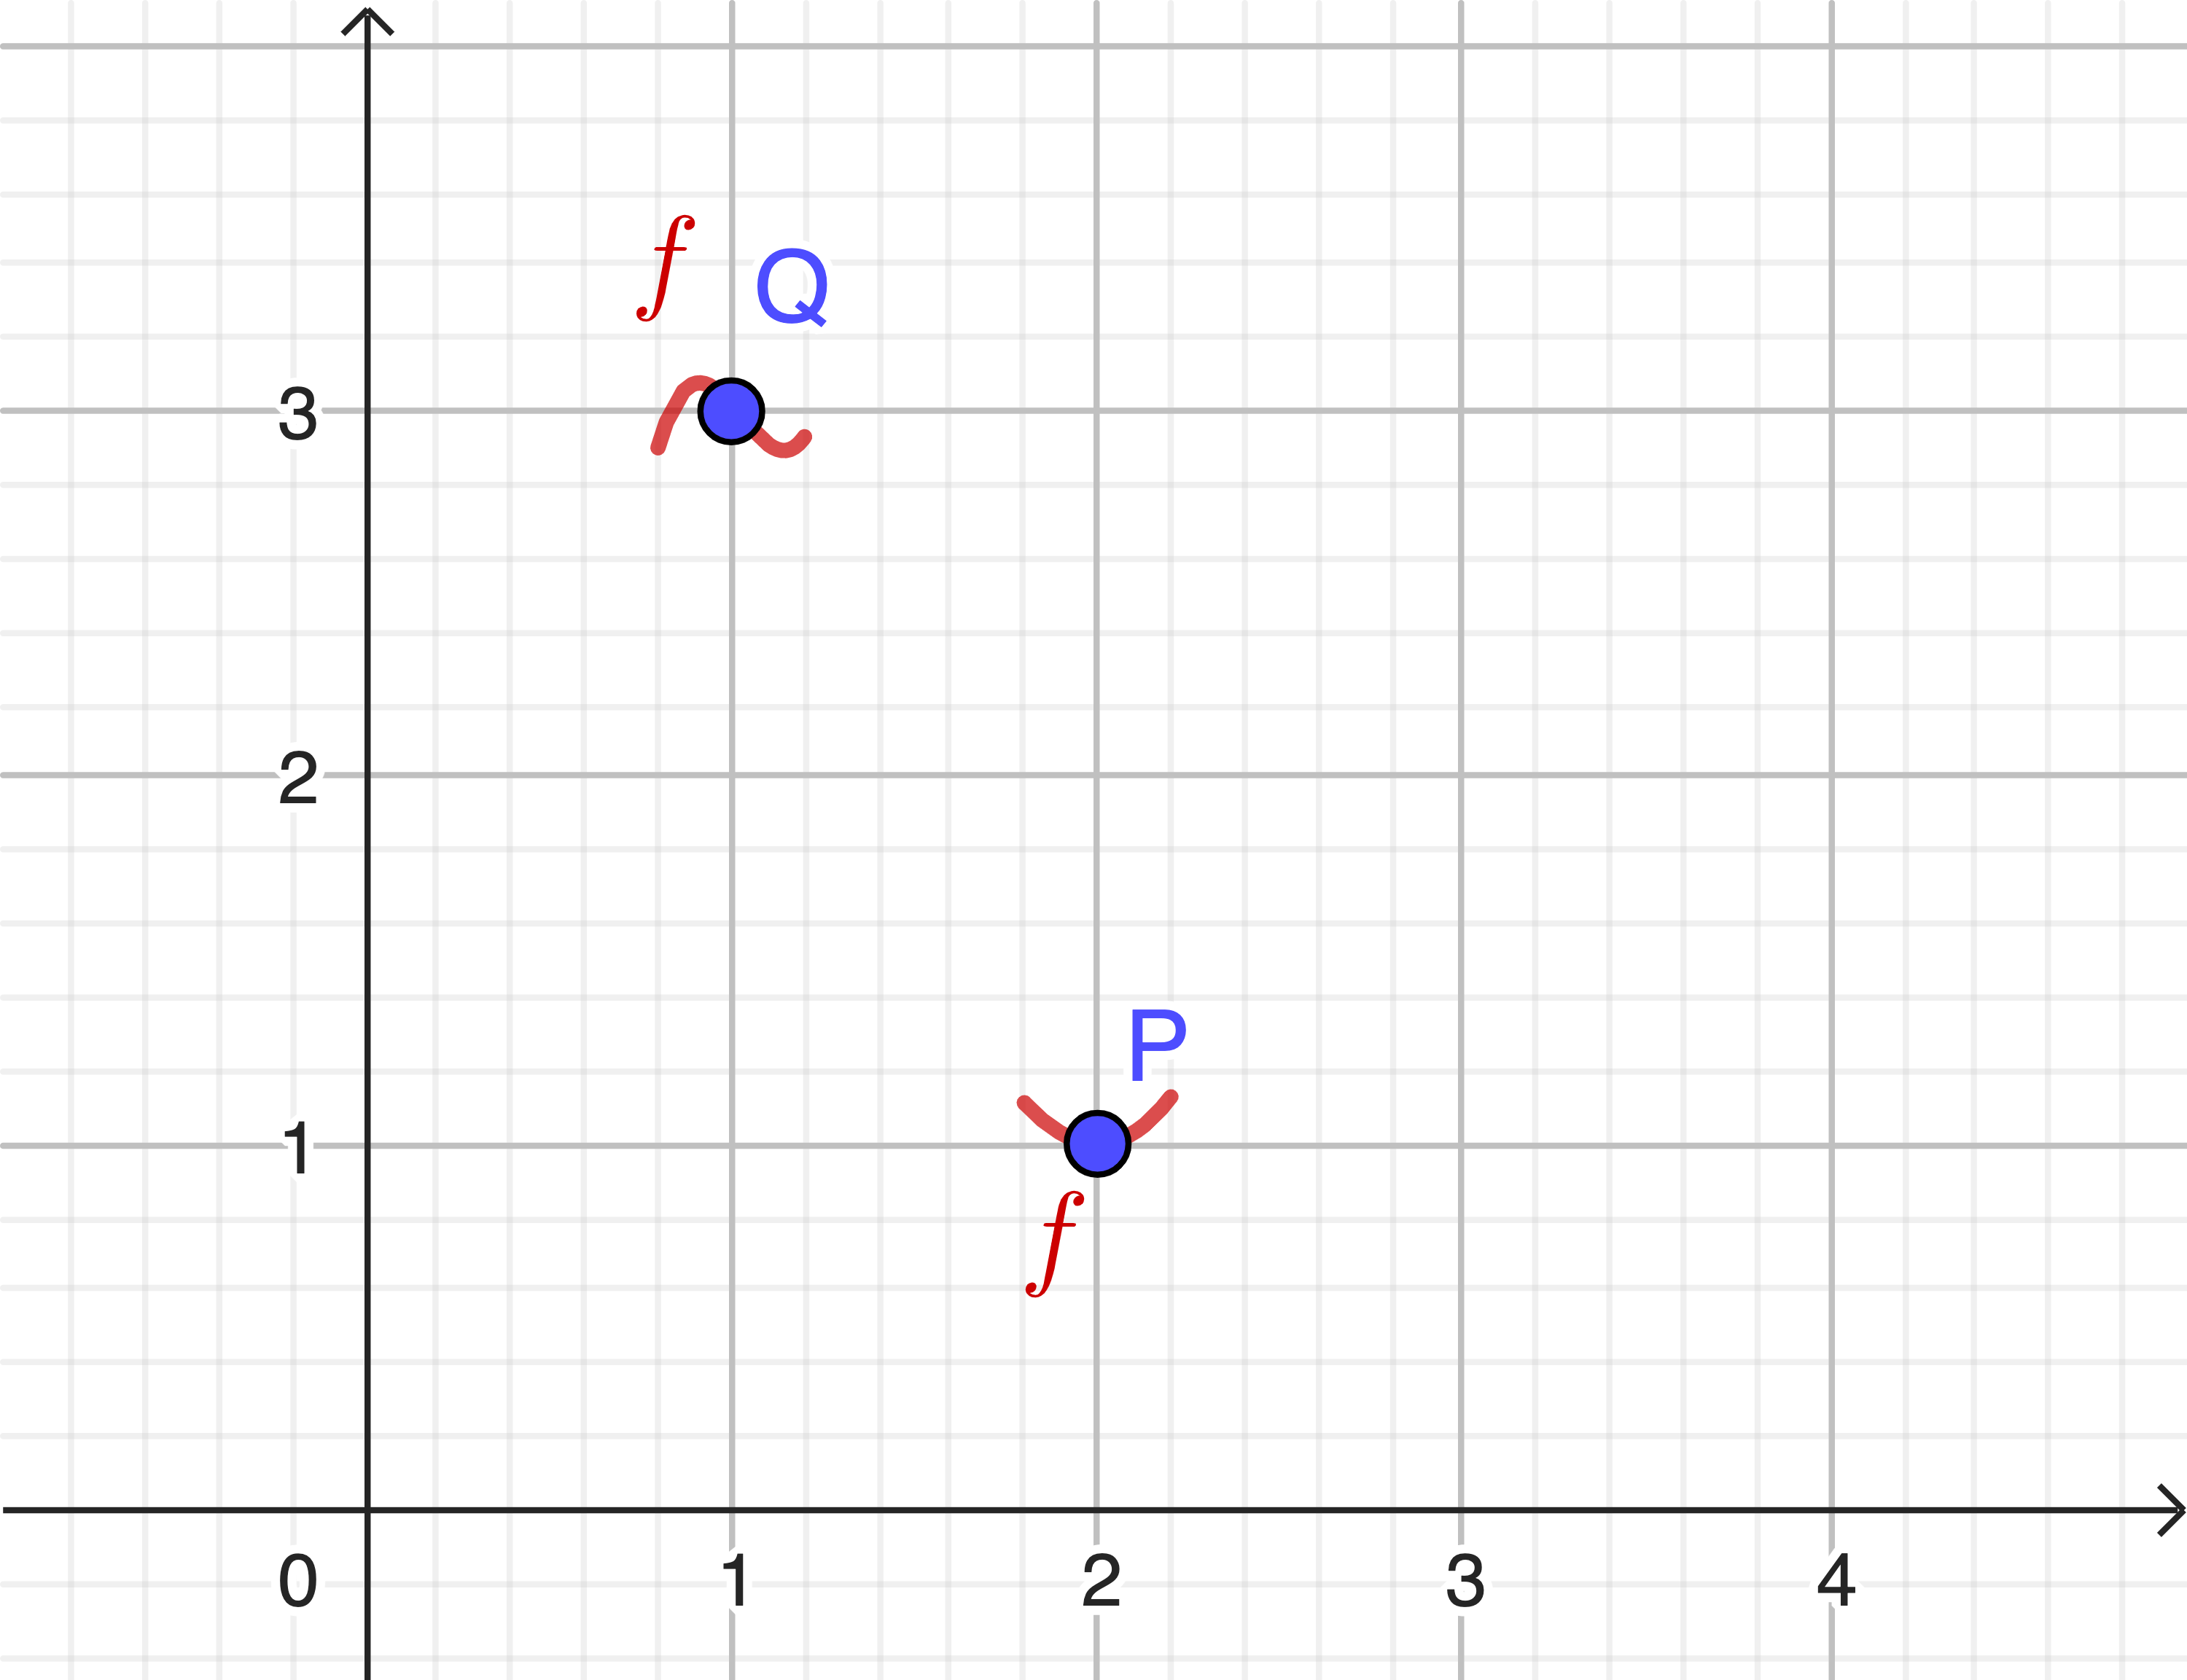
\includegraphics[scale=0.8]{media/fuBest.png}
	\end{center}

	\vspace*{11cm}


	\pagebreak

	\phantom{hello}

	\vspace*{19 cm}

\end{bsp}

\clearpage
\begin{ueb}{}{}
	\begin{enumerate}
		\item Der Graph einer Polynomfunktion 3. Grades hat im Punkt \( P(2,1) \) einen Terrassenpunkt und schneidet die \( x \)-Achse im Punkt \( A(4,0) \). Bestimmen Sie die Funktionsgleichung.
		\item Der Graph einer Polynomfunktion 4. Grades berührt die \( x \)-Achse bei \( x = 0 \). Im Punkt \( T(3,9) \) ist ein Terrassenpunkt. Bestimmen Sie die Funktionsgleichung.
		\item Der Graph einer Polynomfunktion 3. Grades hat einen Wendepunkt bei \( W(1,2) \) und berührt die \( x \)-Achse bei \( x = 2 \). Bestimmen Sie die Funktionsgleichung.
		\item Bestimmen Sie eine Polynomfunktion 3. Grades mit einer Nullstelle bei \( x = -2 \). Der Punkt \( P(0,y_P) \) ist ein Wendepunkt und die Wendetangente \( t \) hat die Gleichung \( y = \frac{1}{3}x +2 \).
		\item Wie lautet die Gleichung der Polynomfunktion 5. Grades, deren zum Ursprung punktsymmetrischer Graph in \( P(1,8) \) einen Terrassenpunkt hat?
		\item Eine zum Ursprung punktsymmetrische Polynomfunktion 3. Grades hat im Punkt \( M(3,-6) \) ein Minimum. Bestimmen Sie die Funktionsgleichung.
		\item Bestimmen Sie \( a \) so, dass der Graph der Funktion \( f \) mit
		      \[
			      f(x) = \frac{1}{2}(x^4 - ax^2)
		      \]
		      bei \( x = 1 \) einen Wendepunkt hat. Wo liegt der andere Wendepunkt? Bestimmen Sie auch noch die Extrema.

		      % \item Eine Polynomfunktion \( f \) hat an der Stelle \( x = 1 \) eine doppelte Nullstelle und es ist \( f''(x) = 6x \). Bestimme die Gleichung dieser Polynomfunktion und zeichne ihren Graphen.

		      % \item Bestimme die Gleichung einer Funktion \( f \) mit einem lokalen Maximum im Punkt \( (1\,|\,1) \) und einem lokalen Minimum im Punkt \( (-1\,|\,-1) \).

		\item  Bestimmen Sie die Gleichung von \( f \), wenn der Übergang vom Parabelbogen zur Strecke \( s \) an der Stelle \( (2, 0) \) knickfrei ist.
		      \begin{center}
			      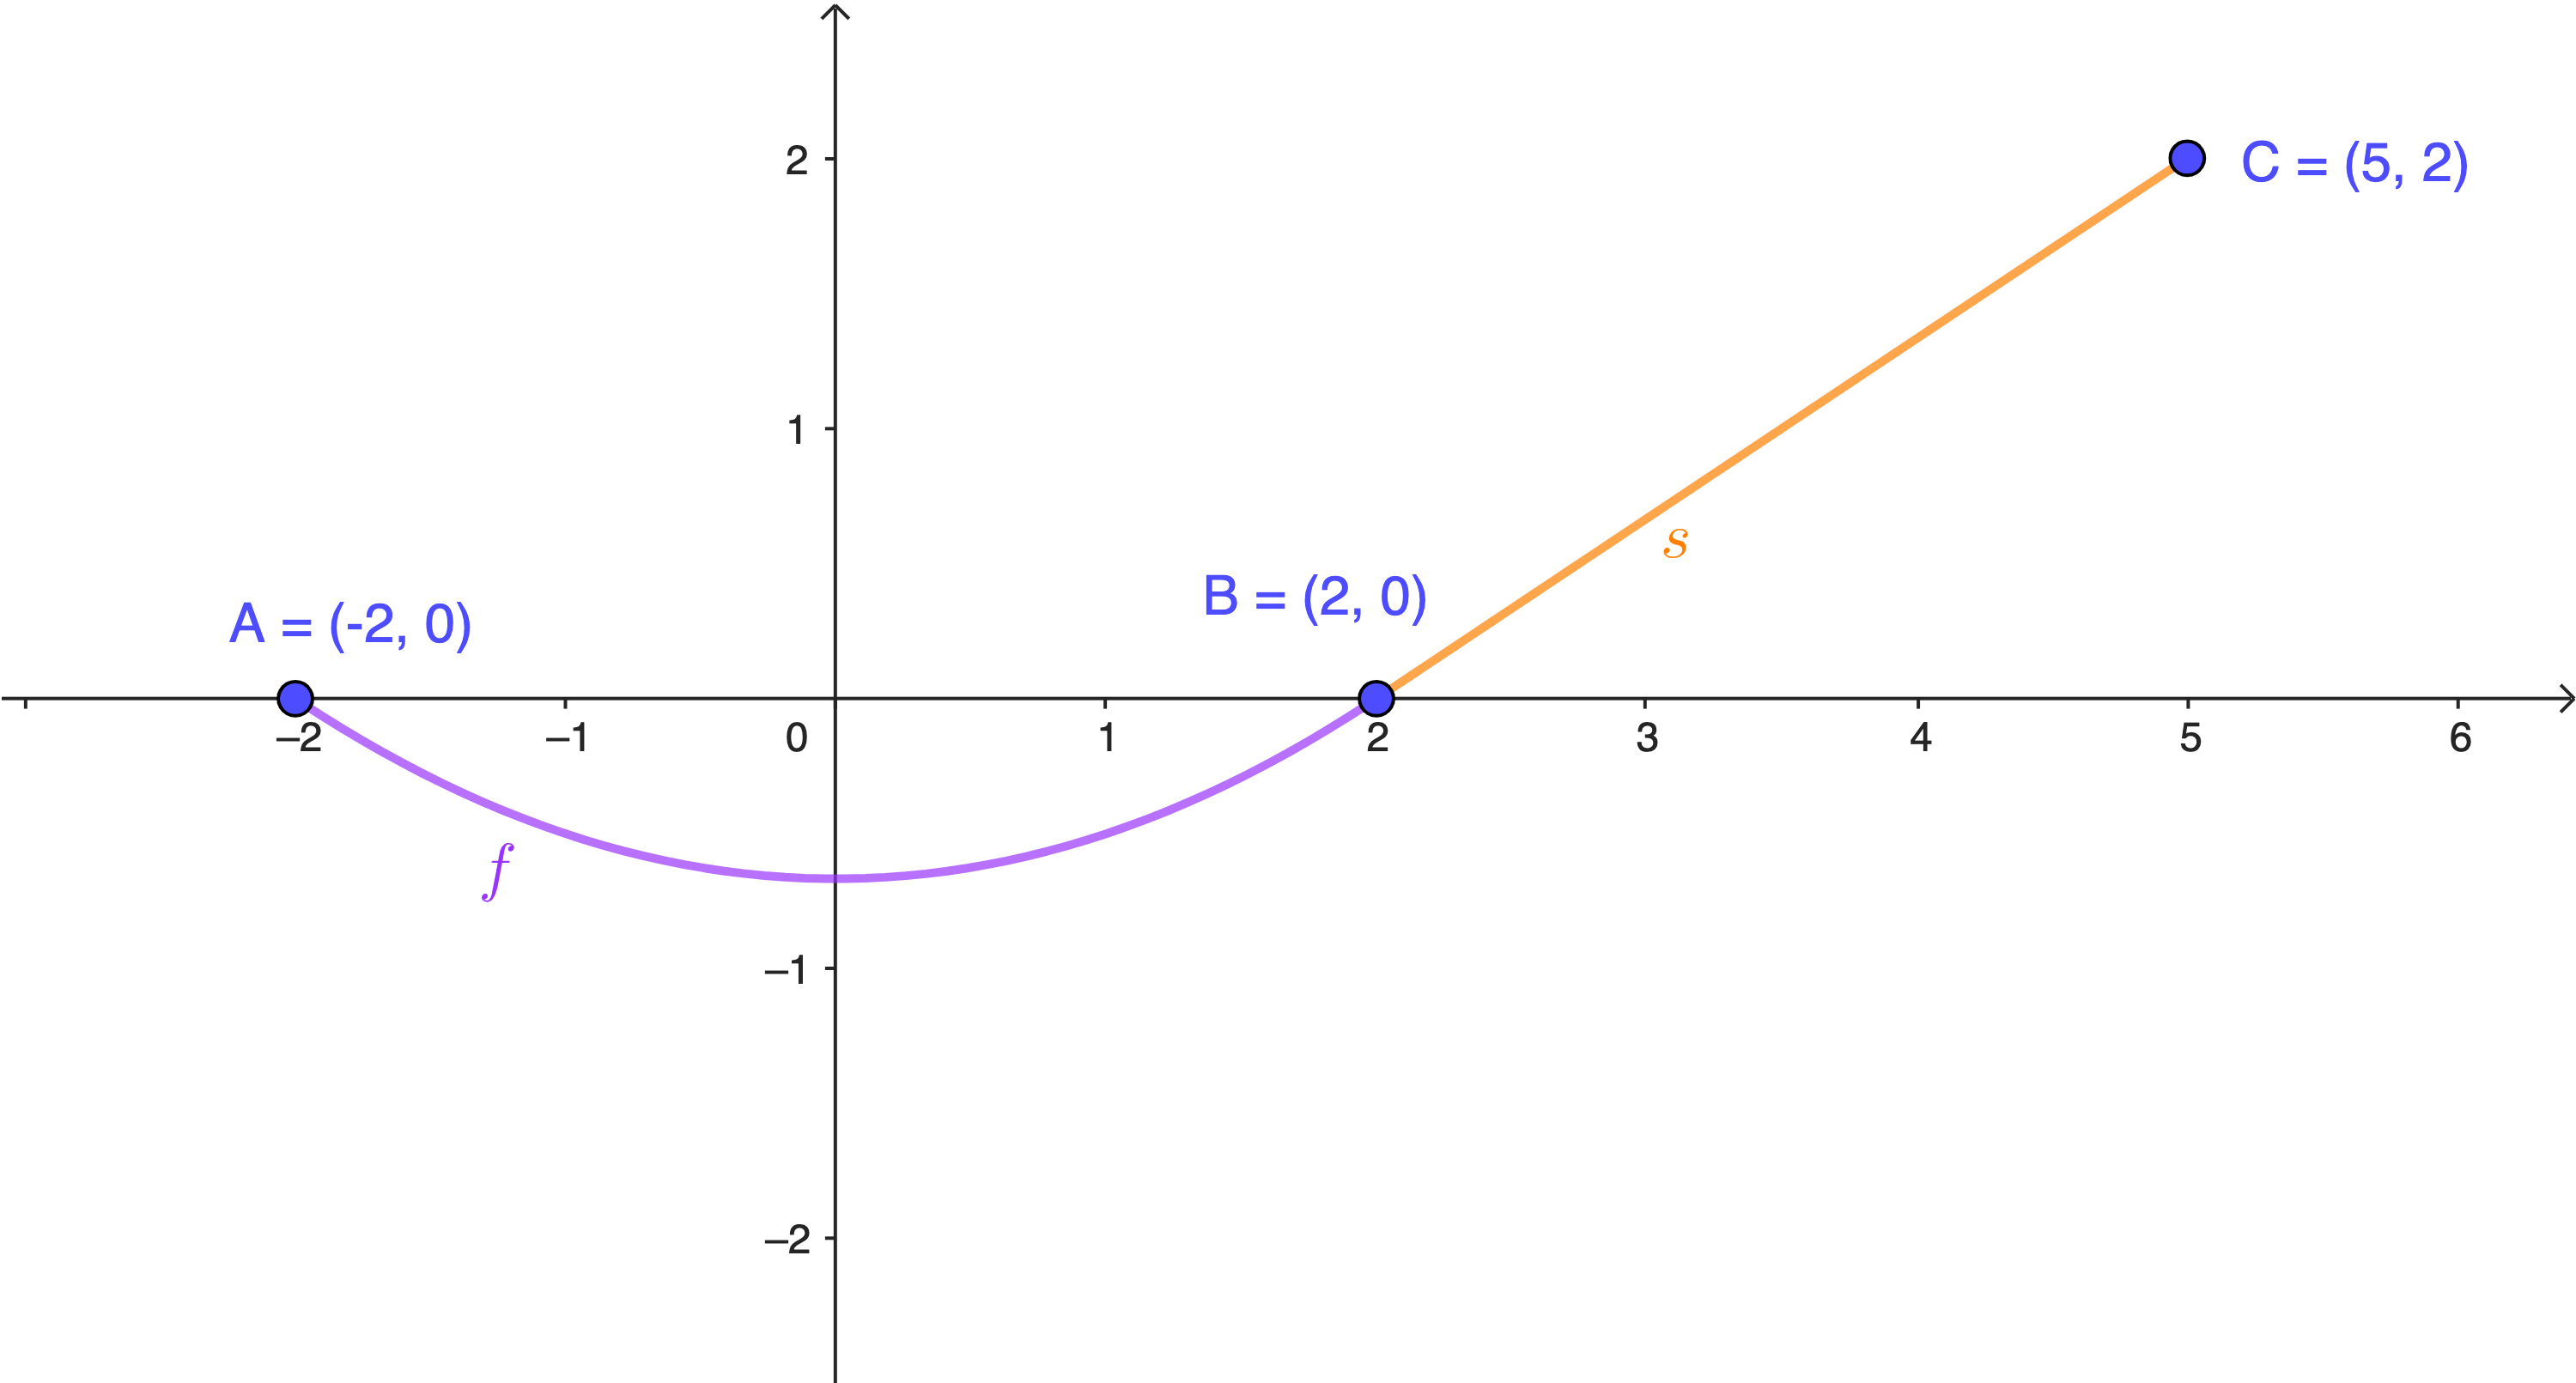
\includegraphics[width = 0.6 \textwidth]{media/knickfrei.png}
		      \end{center}

		\item Gegeben sind die geradlinigen Strassenabschnitte \( u = P(-3, 2)Q(-1, 0) \) und \( w = R(1, 0)S(5, 2) \).\\
		      Es soll eine krummlinige Verbindungsstrasse \( v \) von \( Q \) nach \( R \) gebaut werden, und zwar so, dass die Übergänge in \( Q \) und \( R \) \emph{knickfrei} werden. Beschreiben Sie den Strassenverlauf von \( v \) mit einer Polynomfunktion 3. Grades, die diese Eigenschaft an den beiden Übergangsstellen \( Q \) und \( R \) in die daran anschliessenden geradlinigen Strassenabschnitte nach \( P \) respektive \( S \) besitzt.
	\end{enumerate}

\end{ueb}

\clearpage
\emph{Lösungen:}
\begin{enumerate}
	\item \( f(x) = -\frac{1}{8}x^3 + \frac{3}{4}x^2 - \frac{3}{2}x + 2 \)
	\item \( f(x) = \frac{1}{3}x^4 - \frac{8}{3}x^3 + 6x^2 \)
	\item \( f(x) = x^3 - 3x^2 + 4 \)
	\item \( f(x) = \frac{1}{6}x^3 + \frac{1}{3}x + 2 \)
	\item \( f(x) = 3x^5 - 10x^3 + 15x \)
	\item \( f(x) = \frac{1}{9}x^3 - 3x \)
	\item $a=6, W_2 =(-1, -2.5), H=(0,0), T_{1,2} = \left(\pm\sqrt{3}, -\frac{9}{2}\right)$
	\item $f(x) = \frac{1}{6} x^2 - \frac{2}{3}$
	\item $v(x) = \frac{1}{8}\left(-x^3+3x^2+x-3\right)$ Wenn man es geschickt anstellt, ist das Gleichungssystem nicht so schwer \dots
\end{enumerate}

\clearpage
\begin{ueb}
	{Modellierung der Bewegung eines Roboterarms}{}
	Um einen Roboterarm eine gewünschte Bewegung ausführen zu lassen, muss die Geschwindigkeit der Drehachse von 0 Umdrehungen pro Sekunde (U/sec) auf 10 U/sec erhöht werden. Dies muss innerhalb von 4 Sekunden geschehen. Die Geschwindigkeit $v$ ist somit eine Funktion der Zeit $t$. Damit der Roboter bei der Ausführung dieser Operation keinen Schaden erleidet, werden gewisse Anforderungen an diese Funktion gestellt: Die Geschwindigkeit soll sich nicht sprunghaft ändern, und auch die Beschleunigung darf keine Sprünge machen. Am Anfang ist die Beschleunigung 0 U/sec\textsuperscript{2}, und am Schluss soll sie auch wieder 0 U/sec\textsuperscript{2} betragen.

	Dies lässt sich erreichen, indem eine Geschwindigkeitsfunktion der Form
	\[v(t)=at^3+bt^2+ct+d\]
	gewählt wird, um die Bewegung des Roboters zu steuern.
	\begin{enumerate}
		\item Berechnen Sie die Koeffizienten $a,b,c,d$.
		\item Zu welchem Zeitpunkt ist die Beschleunigung maximal? Wie gross sind zu diesem Zeitpunkt die Geschwindigkeit und die Beschleunigung?
		\item Erstellen Sie ein zweites Geschwindigkeitsprofil. Wählen Sie von
		      (0,0) nach (2,6) ein Parabelstück mit dem Scheitelpunkt in (0,0) und ein weiteres Parabelstück von (2,6) bis (4,10) mit Scheitelpunkt in (4,10). Erfüllt Ihr Geschwindigkeitsprofil die gestellten Bedingungen?
	\end{enumerate}

	% \vspace{
	%     10cm
	% }



\end{ueb}
\pagebreak
Lösungen der Aufgabe \glqq Roboterarm\grqq{}
\begin{enumerate}
	\item 	Das Gleichungssystem:
	      \begin{align*}
		      v(0)  & = 0  \\
		      v(4)  & = 10 \\
		      v'(0) & = 0  \\
		      v'(4) & = 0
	      \end{align*}
	      liefert die Lösung $a=-\frac{5}{16}, b=\frac{15}{8}, c=d=0$. Die Funktion lautet also $v(t)=-\frac{5}{16}t^3 +  \frac{15}{8} t^2 $
	\item Die Beschleunigung ist dort maximal, wo die Geschwindigkeit am stärksten ansteigt, also beim Wendepunkt. Die Gleichung $v''(t)=0$ liefert die Lösung $t=2$. Zu diesem Zeitpunkt ist $v(2)=5$ U/sec und $v'(2)=\frac{15}{4}$ U/sec\textsuperscript{2}.
	\item Die Funktion $v_1$ hätte dann die Gleichung $v_1 (t)=\frac{3}{2}t^2$ (mit einem Gleichungssystem). Die Funktion $v_2$ die Gleichung $v_2 (t)=-t^2+8t-6$.
	      Diese Kombination aus zwei Parabeln erfüllt die Bedingungen nicht, weil sich die Beschleunigung bei $t=2$ \glqq ruckartig\grqq{} ändern würde, womit sie nicht stetig wäre. Es gilt nämlich $v_1'(2)=6\neq 4 = v_2' (t)$

\end{enumerate}

\clearpage
\begin{ueb}
	{Aufgaben mit weiteren Funktionstypen}{}
	\begin{enumerate}
		\item Bestimmen Sie die Parameter $a$ und $b$, sodass die Funktion stetig und knickfrei ist.
		      \begin{enumerate}
			      \item $f(x) = \begin{cases}
					            (x^2-2)^3      & x \le 1 \\
					            \frac{ax+b}{x} & x > 1
				            \end{cases}$
			      \item $f(x) = \begin{cases}
					            \frac{x+a}{ax}  & x \le -1 \\
					            \frac{bx}{x+2a} & x > -1
				            \end{cases}$
			      \item $f(x) = \begin{cases}
					            \sqrt{4x-3}     & x > 1   \\
					            \frac{ax}{bx+2} & x \le 1
				            \end{cases}$
			      \item $f(x) = \begin{cases}
					            a\cdot \sin(x)      & x \le \frac{\pi}{6} \\
					            6\cdot \cos(2x) + b & x > \frac{\pi}{6}
				            \end{cases}$
		      \end{enumerate}

		\item Der Graph der Funktion $f\colon y=\frac{p x}{x-2}$ hat bei $x=4$ die Steigung $m=5$. Berechnen Sie den Wert von $p$.
		\item Bestimmen Sie $a$ und $b$ so, dass der Graph von $f\colon y=\frac{a x^{2}+1}{b x}$ in $P(2,1)$ ein Extremum besitzt. (Tipp: Wenn Sie zuerst den Funktionsterm ausdividieren, ist die Ableitung einfacher zu berechnen.)
		\item Der Graph der Funktion $f\colon y=\frac{a x^{2}+b}{x-3}$ besitzt in $P(-1, 4)$ die Steigung $m=-3$. Bestimmen Sie $a$ und $b$ sowie die Gleichung der Tangente in $P$.
		\item Bei $x=4$ besitzt der Graph der Funktion $f\colon y=x\sqrt{a-x}$ ein Extremum. Berechnen Sie den Wert von $a$.
		\item Bestimmen Sie $a$ und $b$ so, dass die Kurve $f\colon y=a x+\sqrt{x+b}$ in $P(3, 10)$ die Steigung $m=7/2$ hat. (Tipp: Beim Gleichungssystem kann man die Unbekannte $b$ eliminierten, indem man $\sqrt{3+b}$ aus der einen Gleichung isoliert und in die andere einsetzt.)
		\item Der Graph der Funktion $f\colon y=a\cdot \sin x + 2x$ besitzt bei $x=\frac{\pi}{3}$ ein Extremum. Berechnen Sie den Wert von $a$.
		\item Bestimmen Sie $a$ so, dass der Graph der Funktion $f\colon y=\cos^{2}x + a\cdot \sin x$ bei $x=\frac{\pi}{4}$ eine Tangente mit der Steigung $m=1$ besitzt.
		      % \item Die Graphen von $f_{1}\colon y=a\cdot \tan x + b$ und $f_{2}\colon y=\sqrt{2}\cdot \sin 3x + 2a$ berühren sich bei $x=\frac{\pi}{4}$.
		      %       \begin{enumerate}
		      % 	      \item Bestimmen Sie $a$ und $b$.
		      % 	      \item Welche Gleichung hat die gemeinsame Tangente bei $x=\frac{\pi}{4}$?
		      %       \end{enumerate}
		      % \item Der Graph der Funktion $f\colon y=\frac{x^{3}-5x+a}{4x^{3}}$ hat bei $x=3$ eine Nullstelle. Ermitteln Sie $a$ und zeigen Sie, dass es keine weiteren Nullstellen gibt.
		\item Für welchen Wert von $a$ und $b$ berührt die Kurve $f\colon y=(x+a)\sqrt{b x}$ bei $x=1$ die Gerade durch $P(4, 1)$ und $Q(-2, -5)$?
		\item Für welchen Wert von $a>0$ schneiden sich die Gerade $g\colon y=a x$ und die Kurve $f\colon y=\sqrt{2-ax}$ in einem rechten Winkel?


		      % Zur Exponentialfunktion:

		\item Berechnen Sie $a$ und $b$ so, dass der Graph der Funktion
		      \[
			      f\colon y=(x^{2}+b)\cdot e^{a x}
		      \]
		      in der Nullstelle $N(3,0)$ die Steigung $m=6 e$ hat.

		\item Die Kurve
		      \[
			      f\colon y=a x^{2}\cdot e^{b x}
		      \]
		      hat bei $x=1$ ein Extremum und bei $x=-\frac{1}{2}$ die Steigung $m=-\frac{3}{2} e$. Bestimmen Sie $a$ und $b$.

		\item Der Graph der Funktion
		      \[
			      f\colon y=(a x+1)\cdot e^{-x}
		      \]
		      hat bei $x=0$ ein Extremum. Berechnen Sie $a$, entscheiden Sie, ob es sich um ein Minimum oder Maximum handelt und berechnen Sie die Koordinaten des Wendepunktes.


	\end{enumerate}
\end{ueb}
\clearpage
\emph{Lösungen}
\begin{enumerate}
	\item Knickfreie, stetige Funktionen
	      \begin{enumerate}
		      \item $a=5, b=-6$
		      \item $a=3/4, b= -1/6$
		      \item $a=1, b=-1$
		      \item $a=-12, b= -9$
	      \end{enumerate}
	\item $p=-10$
	\item $a=1/4, b=1$
	\item $a=b=-8, t(x)=-3x+1$
	\item $a=6$
	\item $a=3, b=-2$
	\item $a=-4$
	\item $a=2\sqrt{2}$
	      % \item $a=-1.5, b = -0.5, t(x)=-3x + \frac{3\pi-8}{4}$
	      % \item $a=-12$
	\item $a=-2, b=4$
	\item $a= \sqrt{2}$

	      % Zur Exponentialfunktion:
	\item $a=1/3, b=-9$
	\item $a=1, b= -2$
	\item $a=1$ Es ist ein Hochpunkt. Der Wendepunkt liegt bei $W(1, 2/e)$.

\end{enumerate}